%==================== chapter3_26.tex ====================

\clearpage
\thispagestyle{plain}

\begingroup
\fontsize{16pt}{19.2pt}\selectfont
\justifying
\XeTeXlinebreakskip=0pt plus 1pt minus 0.5pt
\setlength{\parindent}{1.5cm}
\setlength{\parskip}{0pt}

\begin{figure}[h]
	\centering
	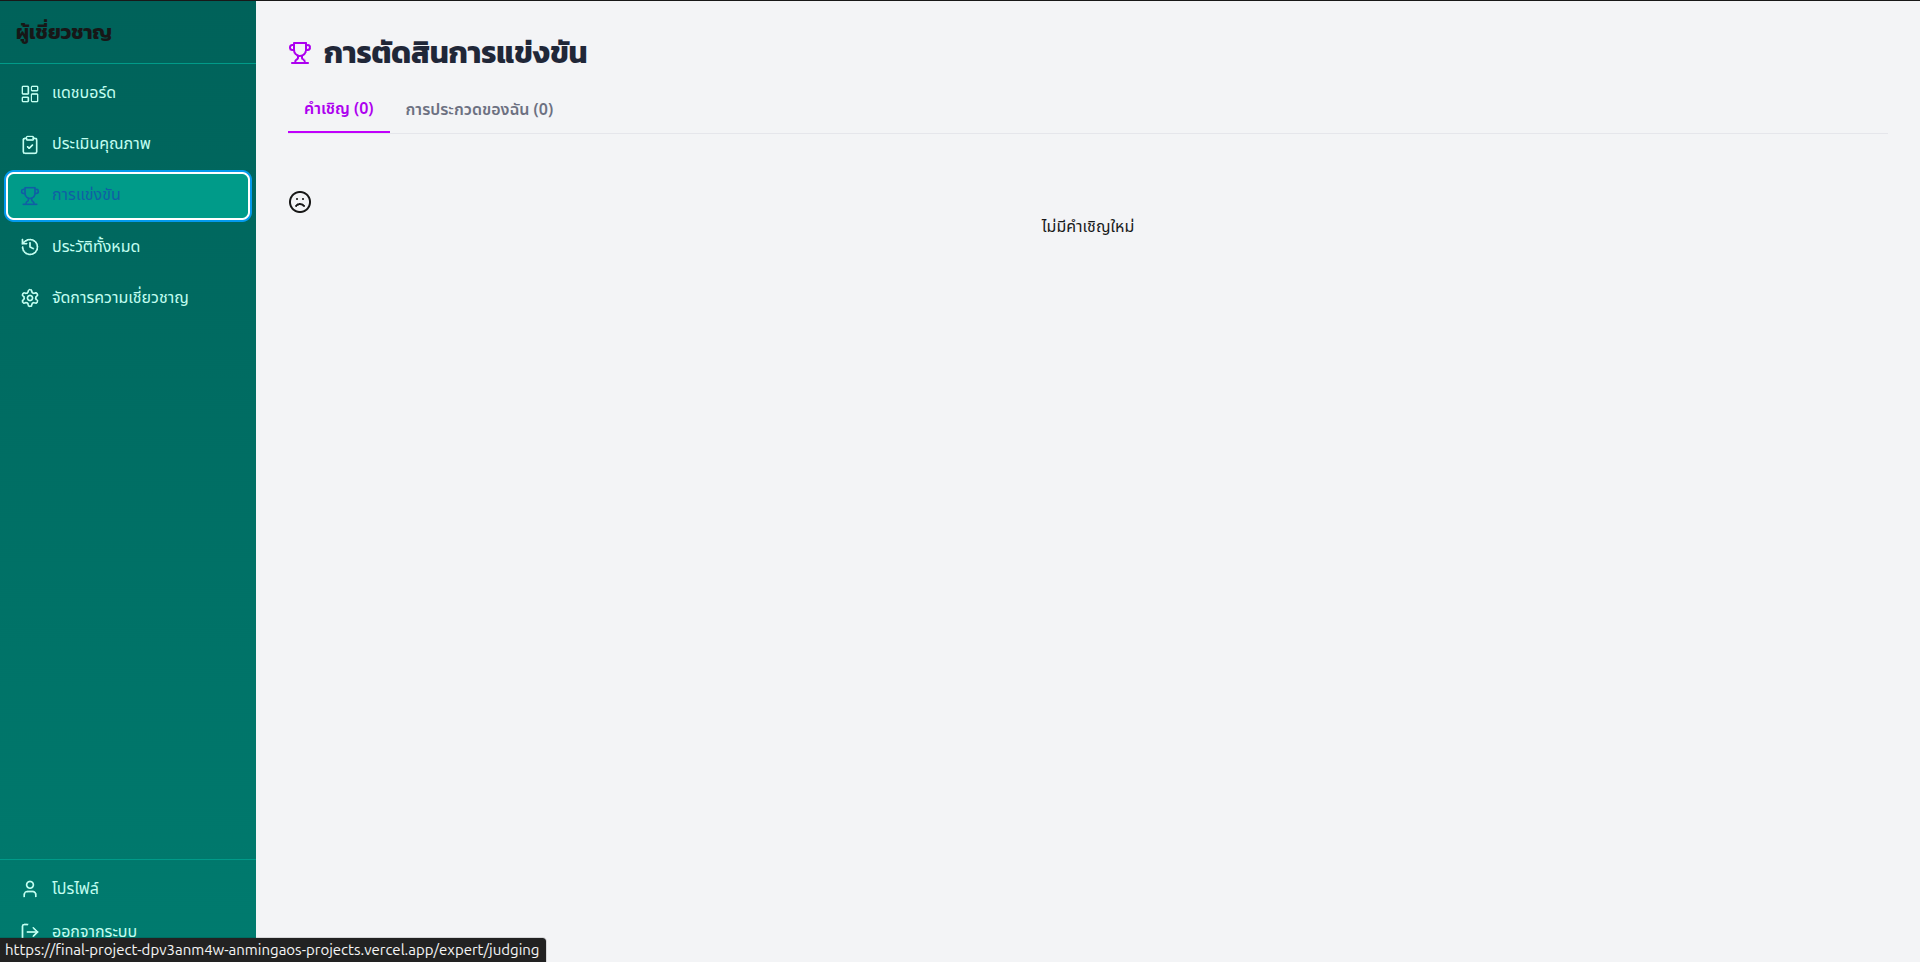
\includegraphics[width=0.8\linewidth]{EP3}
	\caption{หน้ารับงานการเป็นกรรมการ}
\end{figure}

\indent ผู้เชี่ยวชาญจะเห็น รายการคำเชิญใหม่ๆ ที่ผู้จัดการประกวด (Manager) ส่งมาให้เพื่อเป็นกรรมการตัดสิน
ในแต่ละรายการคำเชิญ จะมีปุ่มให้ผู้เชี่ยวชาญตัดสินใจ คือ "ตอบรับ" หรือ "ปฏิเสธ" คำเชิญนั้นๆ 

\vspace{\baselineskip}

\begin{figure}[h]
	\centering
	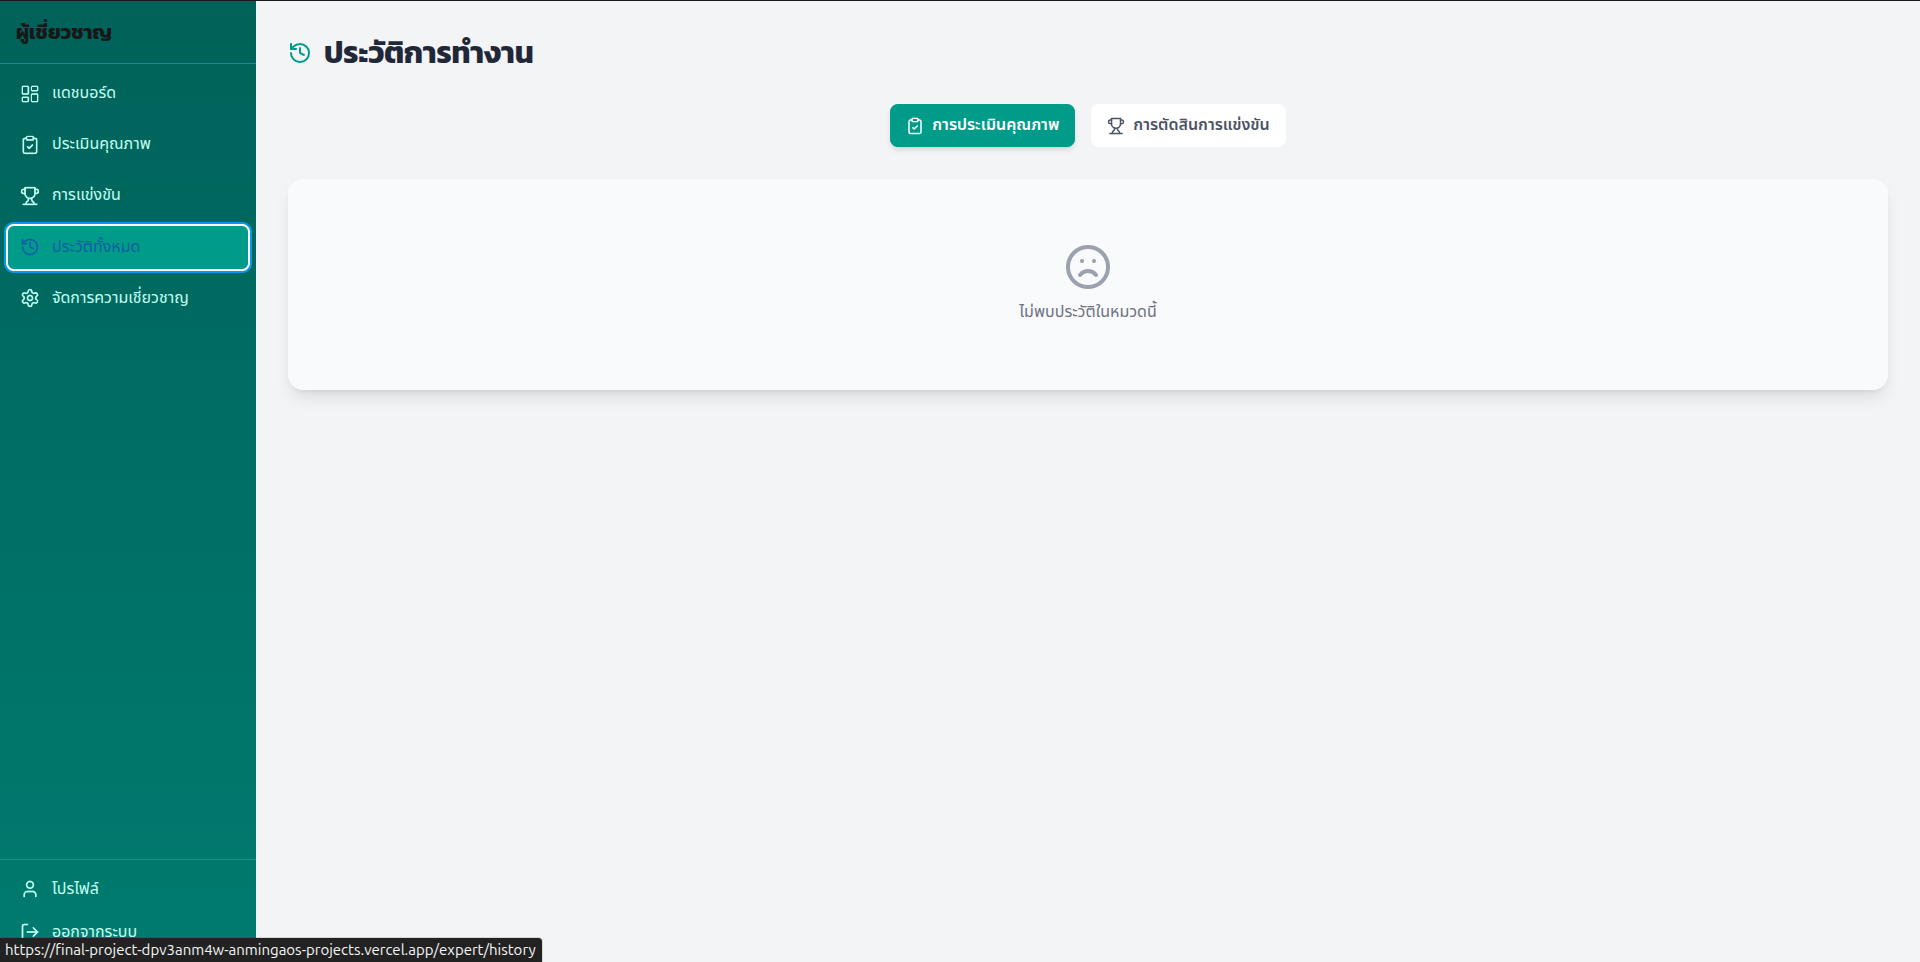
\includegraphics[width=0.8\linewidth]{EP4}
	\caption{หน้าประวัติการทำงาน}
\end{figure}

\indent หน้านี้คือให้ผู้เชี่ยวชาญสามารถ ย้อนกลับมาดูงานทั้งหมดที่เคยทำเสร็จไปแล้วโดยจะมีการแบ่งประวัติออกเป็น 2 ประเภท ซึ่งผู้ใช้สามารถกดเลือกดูได้จากปุ่มด้านบน การประเมินคุณภาพ เมื่อกดปุ่มนี้ (ซึ่งเป็นหน้าที่แสดงในรูป) ผู้เชี่ยวชาญจะเห็น รายการปลากัดที่เคยประเมินคุณภาพไปแล้วทั้งหมด ในรูปแบบตาราง การตัดสินการแข่งขัน 
ถ้ากดปุ่มนี้ ผู้เชี่ยวชาญก็จะเห็น รายชื่อการแข่งขันทั้งหมดที่เคยเข้าไปเป็นกรรมการตัดสิน

\newpage

\begin{figure}[h]
	\centering
	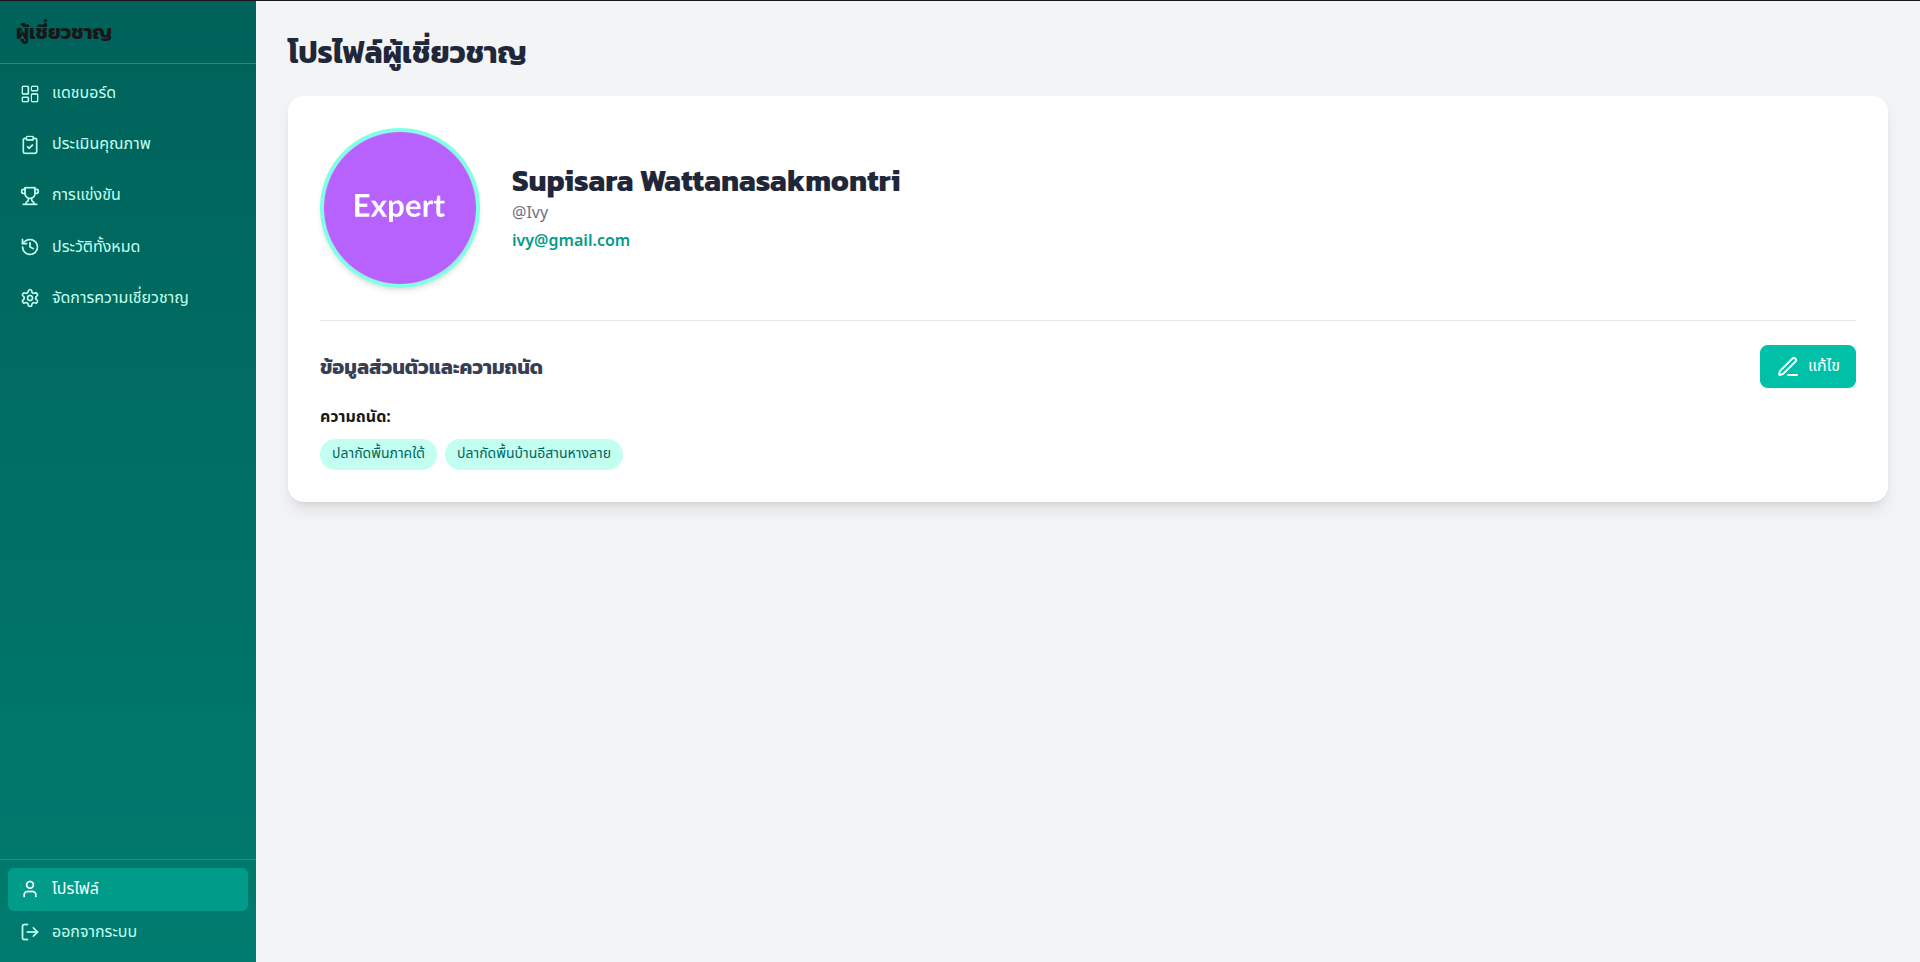
\includegraphics[width=0.8\linewidth]{EP5}
	\caption{หน้าโปรไฟลืผู้เชี่ยวชาญ}
\end{figure}

\indent  เชี่ยวชาญสามารถ ดูและจัดการข้อมูลส่วนตัวของตัวเอง ได้ โดยจะแบ่งการทำงานเป็น 2 ส่วนหลักๆ การดูข้อมูล ในตอนแรกที่เข้ามา ผู้เชี่ยวชาญจะเห็นข้อมูลของตัวเองที่แสดงอยู่ ได้แก่ รูปโปรไฟล์, ชื่อ-นามสกุล, Username และอีเมล ความถนัด (Specialities) จะมีป้าย Tag แสดงประเภทปลากัดที่ตัวเองมีความเชี่ยวชาญเป็นพิเศษ 

\endgroup